\documentclass[12 pt]{uncw_thesis}
%
% Packages
%
\usepackage{amsmath, amssymb, amsthm} % AMS packages
\usepackage{setspace}    % Needed for multiple spacing (single and double)
\usepackage{graphicx}    % Needed for images
\usepackage{epstopdf}     % Use to convert eps images
\usepackage{afterpage}   % Needed to make figures and tables on separate pages
\usepackage{indentfirst} % Use to indent first paragraphs
\usepackage{url}
\usepackage{longtable}
\usepackage{tikz}        % Package for drawing figures
\usepackage{hyperref}    % Needed for live links
\usepackage{lipsum}  
\hypersetup{
    %bookmarks=false,%
    colorlinks,%
    citecolor=black,%
    filecolor=black,%
    linkcolor=black,%
    urlcolor=black
}                        % Eliminate colored links See http://en.wikibooks.org/wiki/LaTeX/Hyperlinks
\urlstyle{same}          % Makes links same font aas text
    % Generate dummy text for sample thesis
%
% Formatting
%
\usepackage{color}
\usepackage{array}
\usepackage{wrapfig}
\usepackage{listings}
\newcolumntype{M}[1]{>{\centering\arraybackslash}m{#1}}
\doublespacing
\oddsidemargin=.54in
\topmargin = -.48in
\textwidth = 5.92in \setlength{\textheight}{8.9in}


% Math environments
\usepackage{amsthm}
\theoremstyle{plain}
\newtheorem{theorem}{Theorem}
\newtheorem{lemma}{Lemma}
\newtheorem{corollary}{Corollary}

\theoremstyle{remark}
\newtheorem*{remark}{Remark}

\theoremstyle{definition}
\newtheorem{definition}{Definition}
\newtheorem{example}{Example}

% ******************************************************************


% Used for forced indentation
\newenvironment{myindentpar}[1]%
{\begin{list}{}%
         {\setlength{\leftmargin}{#1}}%
         \item[]%
}
{\end{list}}

% \numberwithin{equation}{subsection}  %Uncomment for Equation Numbering by Subsection

%
% Start of Document
%
\begin{document}
\pagenumbering{roman}
%
%  TITLE PAGE
%
\pagestyle{empty}
\begin{singlespace}
\begin{center}
     \hskip 1pt \\    % Title on Line 2 - 15 words or fewer
     {\large MORTGAGE LOAN VALUE PREDICTION WITH MACHINE LEARNING}\\
     \hskip 1pt \\
     by \\
     \hskip 1pt \\    % Name on line 6
     Thomas R. Billman III
\end{center} % Start statement on line    
     A paper submitted in partial fulfillment of the requirements to complete Honors in
     the Department of Mathematics and Statistics. \\
     \hskip 1pt \\
     \hskip 1pt \\
\hspace*{3.25in} Approved By: \\
Examining Committee: \\ 
\hspace*{3.25in} \rule{6.5cm}{.01in}\\ %Was originally 3 inch rule
\hspace*{3.25in} Dr. Yishi Wang \\ 
\hspace*{3.25in} Faculty Supervisor \\ 
\rule{7.5cm}{.01in}\\
Dr. Zhuan Ye \\ 
\\ 
\rule{7.5cm}{.01in}\\ 
Dr. Joseph Farinella \\ 
\\
\hspace*{3.25in} \rule{6.5cm}{.01in}\\ % Was originally 3 inch rule
    \hspace*{3.25in} Dr. Zhuan Ye \\
    \hspace*{3.25in} Chair, Mathematics and Statistics \\ 
    \\
    \\
    \rule{7.5cm}{.01in}\\
     Honors Council Representative \\
    \\ 
    \\
    \rule{7.5cm}{.01in}\\
     Director of the Honors Scholars College \\
\begin{center}   
    \hskip 1pt \\
    \hskip 1pt \\    % UNCW on line
    University of North Carolina Wilmington\\
    \hskip 1pt \\    % UNCW on line
    Wilmington, North Carolina \\
    \hskip 1pt \\    % Year on line 
    April, 2017\\
\end{center}
\end{singlespace}
\newpage

%
% Table of Contents
%

\newpage
\pagestyle{plain}
\begin{center}
\tableofcontents
\end{center}


%
% Abstract
%

\sectionx*{ABSTRACT}
\addcontentsline{toc}{section}{ABSTRACT}
This project investigates relationships between mortgages' net present values (NPV) and their related covariates through public datasets from Freddie Mac. These datasets contain loan records for single family houses with 30 year fixed interest rates. To our knowledge, this is the first effort of such investigations on this complexly structured dataset. Given the size of the datasets as well as the complexity of the problem, our investigation begins with cleaning and calculating NPV’s based on each loan’s records, both effectively and efficiently on high performance computing clusters provided by the Texas Advance Computing Center. Classical statistical methods and contemporary machine learning algorithms are deployed for regression and classification. Computation results suggest that machine learning algorithms outperform classical regression and classification methods.

\newpage
\pagenumbering{arabic}
\section{Introduction}
\thispagestyle{plain}
Our research primarily focuses on using contemporary machine learning techniques to  predict mortgage values more accurately than classic linear methods. Previous research has focused on classifying loans at time of origination as prepaid, paid as planned, or default \cite{Deng}.Through literature review, we find related work, but nothing using the Net Present Value (NPV). While it is important to predict the end state of a loan, banks may have a greater interest in profitability prediction. As a proxy for profit, we compute each loan's NPV which adjusts all payments to the time the loan was issued. This is different way to compare the financial impact of loans as opposed to end state classification methods. Additionally, once NPVs are calculated we predict them using data collected at time of loan origination. 

\section{Literature Review}
A mortgage is a loan that is secured by real estate \cite{Fannie}. If a borrower stops making payments on their loan it goes into default, and the bank can foreclose on the property. Through the process of foreclosure, the bank  that  wrote the mortgage claims the property from the borrower. The bank then sells the property and uses the proceeds to recover the rest of the loan's outstanding balance. If the property has dropped in value, it is possible that the bank can lose large sums of money by writing mortgages, so it is important to make sure banks select borrowers who are likely to make their payments. Due to the high financial stakes, the ability to determine which borrowers are mortgage-worthy is very important and the subject of much research. One project used contemporary machine learning techniques to model whether loans will carry out as planned, end in default, or end prepaid \cite{Deng}. This project considered methods such as Binary Logit, Multinomial Logit, K-Nearest Neighbors, K-fold Cross Validation, and Random Forest. Of the models considered, the most accurate model was Random Forest (RF) classification. This model could classify loans into the correct end state with 93\% accuracy. Due to the proven accuracy of RF classification, we decided to use RF modeling in our analysis \cite{Deng}. \\ 
Another project involved an unprecedented dataset of 120 million prime and subprime mortgages from 1995 to 2014 \cite{Sirignano}. After adding local micro and macroeconomic metrics to their dataset, neural networks were used to predict how many loans would end as either prepaid or default within random portfolios of thousands of loans. Their research showed that neural networks considerably outperformed similar analysis using traditional logit techniques. This is particularly impactful for agencies that package and sell mortgage-backed securities as it can drastically improve their methodology of choosing loans for their products. This is also a good indicator for our project, that machine learning algorithms will yield better predictions of NPV as compared to linear regression.
\section{Our Dataset}
Our dataset was obtained from the Federal Home Loan Mortgage Corporation, better known as Freddie Mac, which is a public government-sponsored enterprise. We used their Single Family Loan Level Dataset, which lists origination and performance data for loans based on financial quarter of origination \footnote{The dataset can be found at \href{ http://www.freddiemac.com/research/datasets/sf\_loanlevel\_dataset.html}{http://www.freddiemac.com/research/datasets/sf\_loanlevel\_dataset.html}, and only registered accounts can download it}. The dataset is composed of two files where the first file lays out the details of each loan's origination. It contains 391,419 observations of 26 variables, which are: 
\begin{center}
	\begin{longtable}{ |M{5.5cm}|M{8.75cm}| }
		\hline
		Credit Score & A number summarizing the borrower's creditworthiness and prepared by third parties\\ \hline
		First Payment Date & Date of the first scheduled payment\\ \hline
		First Time Homebuyer Flag & Indicates if an individual is 1) Purchasing the mortgaged property, 2) will reside in the property as primary residence, 3) does not have ownership interests in other residential properties \\
		\hline
		Maturity Date & Date of the final scheduled payment\\
		\hline
		Metropolitan Statistical Area & Similar to Zip Codes, but for large metropolitan areas containing 2.5 million people or more. These are defined by the US Census\\
		\hline
		Mortgage Insurance Percentage & Percentage of loss coverage on the loan, to be paid to Freddie Mac in the event of a default\\
		\hline
		Number of Units & Number of properties covered by this mortgage\\
		\hline
		Occupancy Status & Denotes whether the home is owner occupied, a second home, or investment property\\
		\hline
		Original Combined-Loan-to-Value & Original mortgage loan amount plus possible second mortgage amount divided by initial property value\\ 
		\hline
		Original Debt-to-Income Ratio & Borrower monthly income divided by monthly mortgage payment \\
		\hline
		Original Unpaid Balance (UPB) & Initial amount loaned in the mortgage note\\
		\hline
		Original Loan-to-Value & Initial mortgage loan amount divided by initial property value\\
		\hline
		Original Interest Rate & Original rate indicated on mortgage note\\
		\hline
		Channel & What type of organization sold Freddie Mac this loan (Retail, Broker, etc.)\\
		\hline
		Prepayment Penalty Flag & Indicates if the borrower is penalized for prepayment\\
		\hline
		Product Type & All entries are Fixed Rate Mortgages\\
		\hline
		Property State & The U.S. State the property is located in\\
		\hline
		Property Type & Indicates property type (Single-Family Home, Condo, Co-op, etc) \\
		\hline
		Postal Code & First three numbers of the property's Zip Code\\
		\hline
		Loan Sequence Number & Unique identifier assigned to each loan \\
		\hline
		Loan Purpose & Indicates if the loan is to purchase the house, or refinance the property\\
		\hline
		Original Loan Term & Number of payments calculated from First Payment Date and Maturity Date \\
		\hline
		Number of Borrowers & Number of Borrowers obligated to repay the mortgage (1 or $>$1)\\
		\hline
		Seller Name & Entity who sold the loan to Freddie Mac\\
		\hline
		Servicer Name & Entity who is currently servicing the loan on Freddie Mac's behalf\\
		\hline
		Super Conforming Flag & Loans that exceed conforming loan limits\\
		\hline
		Pre-HARP Loan Sequence Number & Links a HARP loan to its pre-HARP origination data\\
		\hline
	\end{longtable}
\end{center}
\begin{flushleft}
This is the data we will be using to predict NPV, as it is all collected during the loan selection process.
\end{flushleft}
The second file of the dataset contains monthly performance data for each loan. Each loan has an entry for every month recording the status of the loan. This file has 2,311,802 observations of the following 23 variables:
\begin{center}
	\begin{longtable}{ |M{6cm}|M{8cm}| } 
		\hline
		Loan Sequence Number &  Same number found in origination file and used to link the two\\
		\hline
		Monthly Reporting Period & Current Month of entry\\ 
		\hline
		Current Actual UPB & Mortgage ending balance for the  monthly reporting period. It includes scheduled and unscheduled principal reductions\\
		\hline
		Current Loan Delinquency Status& Continuous number of months since Due Date of Last Paid Installment (DDLPI)\\
		\hline
		Loan Age & Number of months since the origination of the loan \\ 
		\hline
		Remaining Months to Legal Maturity & The remaining number of months until the mortgage Maturity Date\\
		\hline
		Repurchase Flag & This indicates loans that have been repurchased or made whole\\
		\hline
		Modification Flag & This indicates that the loan has been modified\\
		\hline
		Zero Balance Code & A code indicating why the loan's balance was reduced to zero (1 = Prepaid/Matured Voluntarily, 3 = Foreclosure, etc.)\\
		\hline
		Zero Balance Effective Date & The month in which the event triggering the Zero Balance Code took place \\
		\hline
		Current Interest Rate & The current interest rate on the mortgage after any modifications\\
		\hline
		Current Deferred UPB & Current amount of non-interest bearing UPB (Only occurs in the event of some loan modifications)\\
		\hline
		Due Date of Last Paid Installment (DDLPI)&The date that the loan's scheduled interest and principal payments were paid through, regardless of when last payment was actually made\\
		\hline
		MI Recoveries & Proceeds received from mortgage insurance in the event of default\\
		\hline
		Net Sales Proceeds (NSP)& Amount received from sale of property less selling expenses\\
		\hline
		Non-MI Recoveries& Other proceeds such as tax, insurance, etc. paid to Freddie Mac\\
		\hline
		Expenses & Expenses Freddie Mac bears in the event of foreclosure. This is an aggregation of Legal Costs, Maintenance and Preservation Costs, Taxes and Insurance, and Miscellaneous Expenses\\
		\hline
		Legal Costs & Legal costs associated with sale of property (not included in NSP) in the event of foreclosure\\
		\hline
		Maintenance and Preservation Costs & Costs associated with maintaining property during foreclosure\\
		\hline
		Taxes and Insurance & Cost of taxes and insurance incurred with sale of property\\
		\hline
		Miscellaneous Expenses & Other expenses associated with sale of property \\
		\hline
		Actual Loss & Default UPB - NSP + Delinquent Accrued Interest - Expenses - Recoveries where Delinquent Accrued Interest is the interest owed on payments missed since DDLPI\\
		\hline
		Modification Cost & Costs associated with a rate modification event\\
		\hline
	\end{longtable}
	\vspace{-\baselineskip}
\end{center}
The Actual Loss variable is particularly relevant to our research, as it gives us a comprehensive overview of losses suffered by the bank holding the loan in the event of foreclosure. Between the loan origination and performance data, we can accurately asses how valuable each loan was for the bank at the time it was written and associate that with data collected at origination. It is also important to note that given the time restrictions of our research we only used the first quarter of 1999 as our dataset. We chose first quarter of 1999 because it was the oldest dataset. This gives it a larger proportion of loans that are already in an end state as compared to other sets which will have more loans which are still active.

\section{Net Present Value}
The value of money is driven by the fact that it can be used to purchase goods and services. Therefore, individuals must be compensated to delay consumption. In addition, due to inflation the purchasing power of money decreases with time. Intuitively, we know that fifty years ago a dollar bill could purchase an entire meal and today the same dollar bill may only buy a drink. This concept is known as the time value of money. When evaluating investment, it is necessary to consider the fact that cash flows in different periods have different values.  Investors calculate the net present value (NPV) of the cash flows to determine if an investment is acceptable. The NPV is defined as the present value of the inflows minus the present value of the outflows. A positive NPV indicates that the investment should be accepted since it generates a profit for the firm and a negative NPV indicates that an investment should be rejected since it is not profitable.\\ 
To express this mathematically, we let \(R_t\) represent a cash flow at time \(t\). If money is received, \(R_t\) is positive and if an amount is paid, \(R_t\) will be negative. \((1+i)\) represents amount an investment should appreciate to compensate the lender for the time value of their money for one unit of time \(t\). Also \(i\) represents the effective interest rate for one unit of time. A financial asset consisting of $n$ different cash flows could have its NPV calculated with the following formula:  
\[NPV_{total} = \sum_{t=1}^n \frac{R_t}{(1+i)^t}\]
Because all the cash flows associated with an asset are included, and brought to the present, \(NPV_{total}\) represents what an asset is worth at the present. It is also worth noting that we assume that if the bank did not invest in this loan, they would invest in a 30 year bond instead, as the most comparable financial asset. Because of this, we set our interest rate \(i\) to be the monthly London Inter-bank Offering Rate (LIBOR) from January of 1999. We chose LIBOR as our index because it represents the rate at which a large bank could loan money as a 30 year commitment and is a frequently cited interest benchmark. Since the LIBOR rate was 2.93\% yearly at that time, our monthly rate came out to around .241\%.
\subsection{Our Analysis}
To calculate the NPVs of these loans, we first need to determine whether or not they ended as paid off or with a foreclosure. We began by associating each loan with its corresponding performance entries. Our programs used the value of each loan's Zero Balance Code to determine if the loan was paid off in good standing or foreclosure. These values and their meanings can be found in the dataset user guide\footnote{Data set guide: \href{http://www.freddiemac.com/research/pdf/user\_guide.pdf}{http://www.freddiemac.com/research/pdf/user\_guide.pdf}}. If the Zero Balance Code is not present or marked NA, it is assumed that the loan is still current and assigns the value ``Current''. If the Zero Balance Code is 1, that means that the loan is prepaid, and it is marked ``Prepaid''. Finally, if the Zero Balance Code is 3 or 9, the loan ended in foreclosure and it is marked ``Default''. Once the loan has been classified, it gets put into one of two NPV calculation formulas.
\subsection{Prepaid and Current Loans}
If a loan is either current or prepaid the NPV is calculated with the same function. Due to the fact that many people do not make level payments on their loans, we use the performance data to compute each payment separately. The theory behind this is that each payment has two parts; one part of the payment compensates the bank for the time value of holding the borrower's outstanding balance, and the other part pays down the outstanding balance. This can be referred to as the interest and principal portions of the payment, respectively. Additionally, since this is the only cash flow for the bank at time $t$, it is represented by \(R_t\) in our NPV calculations.  So:
\[R_t = Payment_t = Interest_t + Principal_t\]
We define the outstanding principal, or Current Unpaid Balance, at time \(t\) as \(CUPB_t\). Additionally, since the interest rate \(r\) is quoted as a yearly percent in our dataset (3 for 3\% instead of .03) we have to divide by 1200 to determine the monthly interest rate charged by the bank. It follows that the interest owed in a given monthly payment is the previous CUPB multiplied by the monthly interest rate. Additionally, by checking the difference in CUPB we find the amount the principal was paid down. Mathematically:
\[Interest_t = CUPB_{t-1}*(r/1200)\]
\[Principal_t = CUPB_{t-1} - CUPB_{t}\]
Therefore: 
\[R_t = CUPB_{t-1}*(r/1200) + CUPB_{t-1} - CUPB_{t}\]
And the NPV of all payments is:
\[NPV_{payments} = \sum_{t=1}^n \frac{CUPB_{t-1}*(r/1200) + CUPB_{t-1} - CUPB_{t}}{(1+i)^t}\]
However, to get the total NPV of the loan we need to subtract the original amount lent or Original Unpaid Balance (OUPB). This does not need to be adjusted for time as it was lent at time of origination, yielding us a final:
\[NPV_{total} = NPV_{payments} - OUPB\]
Our analysis will be refer to this \(NPV_{total}\) as just NPV. Our R code reflects this formula for NPV calculation and can be found in my Github Repository\footnote{GitHub Repository: \href{https://github.com/tbillman/Wang499}{https://github.com/tbillman/Wang499}}
\subsection{Default}
In the event that a loan ended in foreclosure, a different NPV formula was required. To find the NPV here, we take a similar approach as in the previous case with one major difference. A defaulted loan has a remaining outstanding balance that was not paid off at the end of their loan. This balance has to be adjusted using all the expenses associated with foreclosing on a home and the net proceeds received by selling the home. 
\[NPV_{total} = \sum_{t=1}^n \left( \frac{CUPB_{t-1}*(r/1200) + CUPB_{t-1} - CUPB_{t}}{(1+i)^t}\right) - OUPB + \frac{CUPB_T + AL}{(1+i)^T}\]

 $CUPB_T$ is the current unpaid balance at time of account closure, and $AL$ represents Actual Loss,  which is given in the dataset. We let $T$ represents the number of months from loan origination to loan  foreclosure. Since $AL$ is listed as a negative number, the cash flow the bank receives at time of account closure would be CUPB + AL. Since this occurs many years into the mortgage, it is important to adjust it back to time of origination. In this case account closure happens \(T\) months after origination. In our code we find $T$ by taking the date of the last payment and adding the number of months it took until account closure. This can be calculated using First Payment Date and Zero Balance Effective Date. This gives us the total number of months between origination and foreclosure. 
\subsection{Application}
Due to the fact that this data is comprised of two files, it was imperative to find an efficient way to match the performance data for each loan to its respective origination data before we could compute each loan's NPV. This was challenging because the number of performance entries for each origination entry is variable. Additionally, due to the size of our dataset we had to solve this problem in an efficient manner. Our first solution that worked utilized a for loop and took roughly 30 minutes to match performance data to 1000 origination entries. Once we switched to an sapply() method, the time was cut to around 10 minutes. Finally, by using matrix operations we could match 1000 origination entries to their performance counterparts in around 10 seconds. We determined that this was fast enough to precess the full dataset in a reasonable amount of time. The R code for this can be found in my Github Repository, but an outline of the process is as follows:
\begin{center}
	\begin{tabular}{|M{6cm}|M{8cm}|} 
		\hline
		Step 1: Read in the datasets & Read both with read.delim()\\ 
		\hline
		Step 2: Look for when the Sequence Number Changes& Subtract each sequence number from the previous entry\\
		\hline
		Step 3: Determine which have differences & Isolate nonzero entries \\
		\hline
		Step 4: Partition performance data into sets by origination file & Use lapply() with our list of sequence number changes\\
		\hline
	\end{tabular}
\end{center}
Finally, once we had our loans classified and developed a formula to compute the NPV in either case, we computed them all. It is also worth noting that we did not compute NPVs of loans that only have one performance file or were marked as repurchased prior to property disposition. These were all minor cases, and not useful for prediction. We added the full list of NPVs as another column to the origination file, and this was used for our regression and classification. 
\section{Geographic Mapping}
Given that our data had the first three numbers of each loan's zip code, we decided to look at how these NPVs look across the country. To do this, we used R packages such as ggplot2, evaluate, mapproj, fiftystater, zipcode, ggmap, and tidyverse. Our code followed this process:
\begin{center}
	\begin{tabular}{|M{6cm}|M{8cm}|} 
		\hline
		Step 1: Load libraries& library(``ggplot2"), etc.\\
		\hline
		Step 2: Read data & read\_csv(``File Location")\\
		\hline
		Step 3: Find representative Zip Code for all leading 3 digits of Zip Codes in our dataset&  00200 $\rightarrow$ 00210,  00500 $\rightarrow$ 00501 ... 99800 $\rightarrow$ 99801,99900 $\rightarrow$ 99901\\
		\hline
		Step 4: Find representative states for all leading 3 digits of Zip Codes in our dataset& 00200 $\rightarrow$ NH, 00500 $\rightarrow$ NY ... 99800 $\rightarrow$ AK, 99900 $\rightarrow$ AK\\
		\hline
		Step 5: Match each entry's Zip Code to it's respective state with our data frame& Entry 1 has Zip Code 19300, is in PA, and has NPV \$-12,008.92\\
		\hline
		Step 6: Compute the mean NPV for each state & AK $\rightarrow$ \$19,284.79, AL $\rightarrow$ \$18,721.94 ...\\ 
		\hline
		Step 7: Compute the standard deviation of NPV for each state & AK $\rightarrow$ \$13,673.22, AL $\rightarrow$ \$15,694.98 ...\\
		\hline
		Step 8: Compute the ratio of mean of NPV and standard deviation of NPV for each state & AK $\rightarrow$ 1.4104, AL $\rightarrow$ 1.1927 ...\\
		\hline
		Step 9: Graph data with ggplot2() & Figures \ref{fig:MapAvg}, \ref{fig:MapSD} and \ref{fig:MapRatio}\\
		\hline
	\end{tabular}
\end{center}
The three graphs we plotted were the average NPV (Figure~\ref{fig:MapAvg}), standard deviation of NPVs (Figure~\ref{fig:MapSD}), and the ratio between the two (Figure~\ref{fig:MapRatio}). Figure ~\ref{fig:MapRatio} is useful for banks looking for the best risk adjusted loan opportunities.
\begin{figure}
	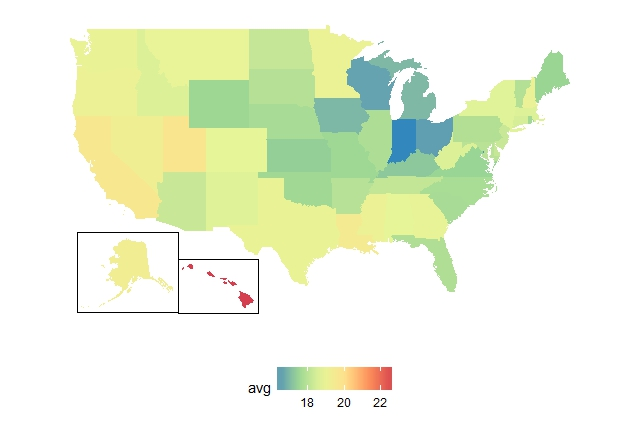
\includegraphics[width=0.9\textwidth]{images/MapAvg.jpeg}
	\caption{Average NPV by state (average scaled by \$1000)}
	\label{fig:MapAvg}
\end{figure}
\begin{figure}
	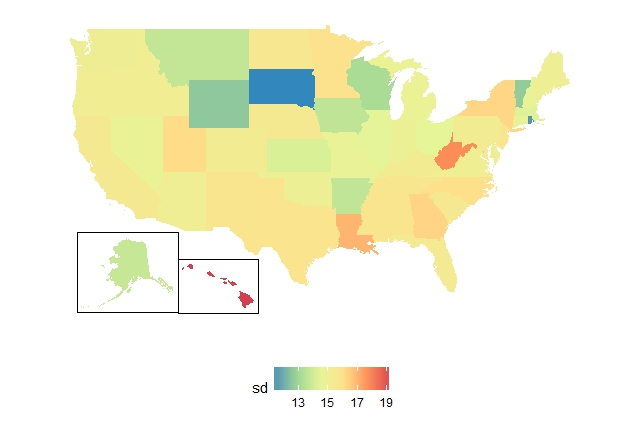
\includegraphics[width=0.9\textwidth]{images/MapSD.jpeg}
	\caption{NPV standard deviation by state (SD scaled by \$1000)}
	\label{fig:MapSD}
\end{figure}
\begin{figure}
	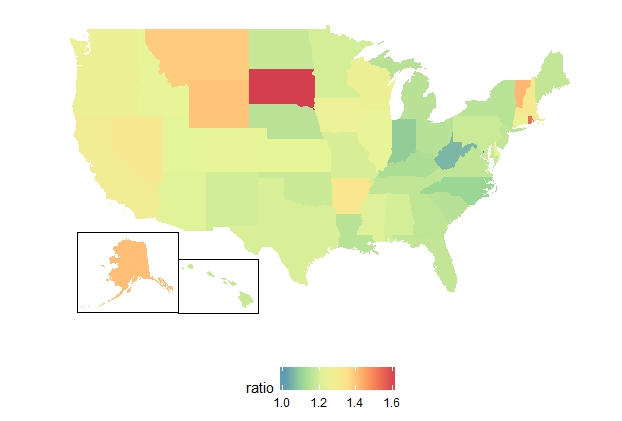
\includegraphics[width=0.9\textwidth]{images/MapSR.jpeg}
	\caption{$\frac{AVG. NPV}{SD(NPV)}$ by state}
	\label{fig:MapRatio}
\end{figure}
\section{High Performance Computing}
Due to the large size of this dataset and the computational requirements of the regression and classification methods we are implementing, access to the Stampede2 supercomputer greatly sped up our ability to run this analysis. Stampede2 is funded by the National Science Foundation, and is the flagship supercomputer at the Texas Advanced Computing Center. Due to the high computing power and memory of the Knights Landing nodes, we could run RF and RGLM analysis on our full dataset in only three hours.  
\section{Linear Regression}
\subsection{Initial Data Cleaning}
\begin{wrapfigure}{r}{0.5\textwidth}
	\vspace{-2cm}
	\centering
	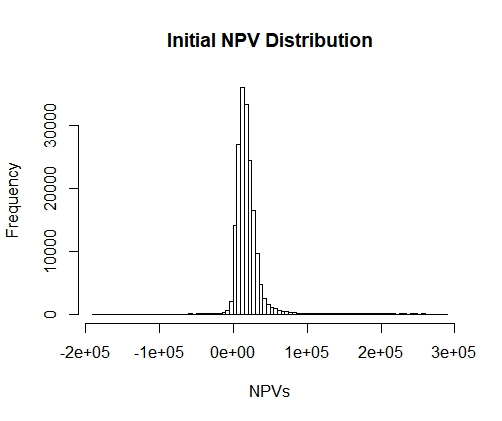
\includegraphics[width=0.45\textwidth]{images/InitalNPVs.jpeg}
	\caption{NPVs of complete cases}
	\label{fig:InitialNPVs}
\end{wrapfigure}
Once we had our NPVs calculated, we began with simple linear regression to see if there was much correlation between the origination data and NPVs. After removing trivial columns with only  one unique value and only keeping rows that had information in all columns, we were left with a 178,058 x 25 matrix. Figure ~\ref{fig:InitialNPVs} shows the initial distribution of the NPVs.  After running an initial linear regression on this data, we obtained an \(R_a^2\) value of .008039, which is very low. Ideally our \(R_a^2\) value would be as close to 1 as possible. Given the strong clustering in the middle, we believed that the presence of outliers on both ends of the curve were effecting our model and that systematically removing them would boost the predictive power of our regression. 
\subsection{Cook's Distance}

\begin{wrapfigure}{l}{0.5\textwidth}
	\vspace{-\baselineskip}
	\centering
	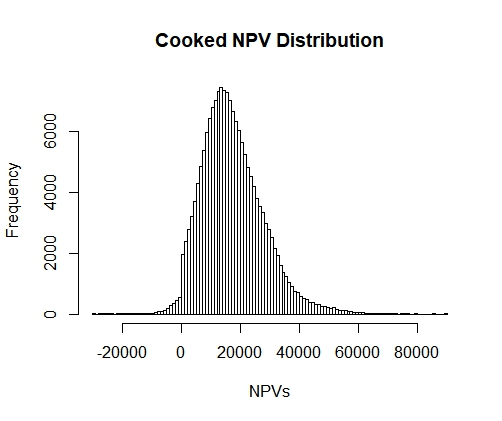
\includegraphics[width=0.4\textwidth]{images/Cooked.jpeg}
	\caption{Entries without outliers}
	\label{fig:Cooks}
\end{wrapfigure}
In order to remedy our outlier problem, we calculated the Cook's Distance of each point. ``Cook's distance, denoted by $D_i$ is an aggregate influence measure, showing the effect of the $i$th case on all $n$ fitted values'':
\[D_i = \frac{\sum_{j=1}^n(\hat{Y_j}-\hat{Y_{j(i)}})^2}{pMSE}\]
Where $\hat{Y_j}$ denotes the predicted value of the $j$th observation and $\hat{Y_j(i)}$ is the predicted value of the $j$th observation where $j \neq i$ and the $i$th observation is removed. Additionally, $p$ represents the number of covariate predictors in our linear regression model, and $MSE$ is the mean squared error of our initial model \cite{512}.
Removing Cook's Distance outliers is useful because our regression is aimed at predicting mortgage values of typical loans, and outlying loans can be considered on a case by case basis. A general rule of thumb is to discard points with distance greater than \(\frac{4}{n}\), and \(n\) is the number of data points \cite{Cook's Rule}. After points with outlying values were removed our new distribution can be seen in Figure~\ref{fig:Cooks}. It is also worth noting that in this distribution there is a large spike right around where NPV = 0. This is because there is a large number of  defaulted mortgages with Actual Loss = 0. This is due to financial regulations where if the bank can recover more than their CUPB and foreclosure costs the remaining proceeds go to the borrower. This leaves many defaults that would have a positive NPV just above 0. After rerunning another linear regression, our \(R^2_a\) value jumped to .01711. However, this is still very low, so we looked to other tactics to improve predictive power.

\subsection{Multi-collinearity}
We also checked for multi-collinearity between our different predictors. ``A formal method of detecting the presence of multicollinearity that is widely accepted is the use of variance inflation factors [VIFs]. These factors measure how much the variances of the estimated regression coefficients are inflated as compared to when the predictor variables are not linearly related'' \cite{512}. This can be expressed quantitatively as follows: 
\[(VIF)_k = (1-R_k^2)^{-1}\]
Where $R_k^2$ is the $R^2$ value of the linear model predicting the covariate $k$ using the remaining $p-1$ covariates. Common tolerance limits for VIF are 10,100, and 1,000 \cite[p.~408-410]{512}. A low VIF indicates low multicollinearity, whereas a high value indicates that certain variables are not important in our linear regression. 
When computing the VIF for all of our variables, all values were below 3 with the exception of Combined Loan to Value Ratio (CLTV) and Loan to Value Ratio (LTV). These variables had VIFs of over 2000. This is because CLTV is only different than LTV if someone refinances their mortgage, which is rare. Since LTV is more useful for loan origination, we kept that variable and removed CLTV from the regression. After removing CLTV, the VIF of LTV dropped below 3, but our \(R^2_a\) value remained similar. This indicates that multicollinearity was not having a significant effect on suppressing our \(R^2_a\) value.
\subsection{Significant Covariates}
\begin{figure}
	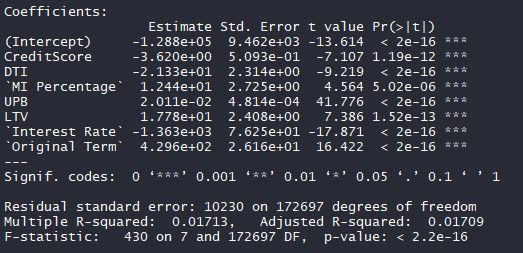
\includegraphics[width=0.9\textwidth]{images/ANOVA.jpg}
	\caption{ANOVA table of Linear Regression}
	\label{fig:ANOVA}
\end{figure}
Figure~\ref{fig:ANOVA} shows all the covariates with $p$ values below .05 after removing Cook's outliers and variables with high VIF. However, a few of the covariate estimates are not immediately intuitive. Particularly, an increase of Credit Score is associated with a decrease in NPV. This is likely because borrowers with high credit score are more likely to prepay their mortgages, resulting in a lower NPV of the mortgage. These borrowers are also more likely to have lower interest rates on their mortgages which further suppresses NPV. Additionally, although a higher interest rate increases payment size Interest Rate has a negative coefficient. We believe this is related to the fact that a higher interest rates are usually given to less qualified borrowers, who are more likely to default on their loans. The rest of the variables seem to be going in an intuitive direction. 

\subsection{Data Transformation}
\begin{wrapfigure}{r}{0.5\textwidth}
	\vspace{-2\normalbaselineskip}
	\centering
	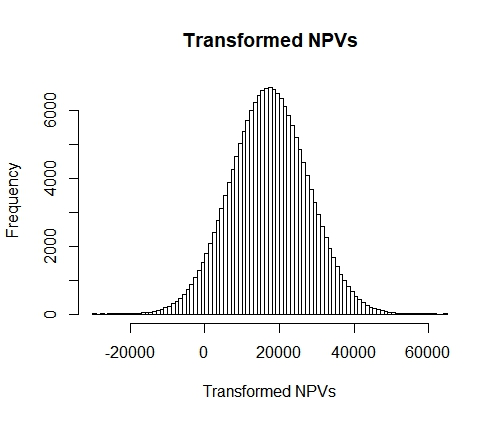
\includegraphics[width=0.4\textwidth]{images/Transformed.jpeg}
	\vspace{-\normalbaselineskip}
\end{wrapfigure}

The final tactic we tried was transforming the data into a normally distributed set. This was to test if the non-normality of our dataset was having an effect on suppressing our predictive power. To do this, we found the percentile of each NPV value, and mapped it to a normal distribution with the same mean and standard deviation as our dataset. To do this we used the ecdf() function in R. However, even after this our \(R_a^2\) value only rose to .01812. After this we concluded that simple linear regression would not have strong enough predictive power on this dataset to be useful.
\section{Random Forest}
\begin{figure}
	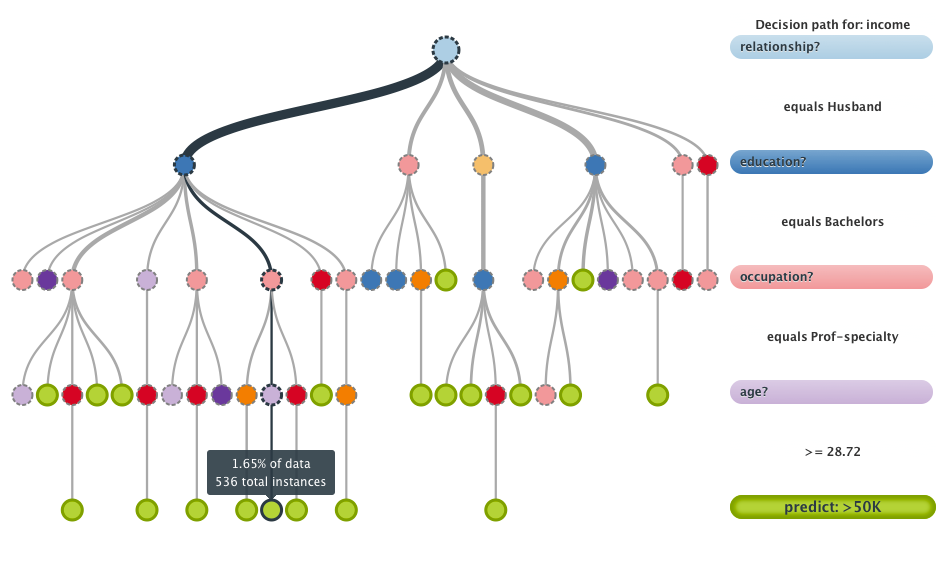
\includegraphics[width=0.9\textwidth]{images/RF.png}
	\caption{An example decision tree for income prediction}
	\label{fig:DecisionTree}
\end{figure}
Random Forest is a contemporary machine learning technique developed by Dr. Leo Breiman at University of California at Berkeley in 2001 \cite{RF}. Fundamentally, RF takes random subsets of the data and uses them to train decision trees. An example of a decision tree can be found in Figure~\ref{fig:DecisionTree}. By training many of these trees on subsets of the data and taking an average of their predictions, we develop a more robust prediction model. This method can be used to predict either continuous or categorical variables. When deciding how to analyze this dataset with RF, we had a few options. Our first attempt was using the dataset to predict NPVs as a continuous variable via regression model. Another option was partitioning the NPV data into categories (Negative, Low, Medium, High) and predicting which NPV category a particular loan would fall into. 

\subsection{Regression}
\begin{figure}
\begin{center}
	\begin{tabular}{|M{5.5cm}|M{8.75cm}|}
		\hline
		Step 1: Remove Degenerate Columns & Columns like Product Type, which only contain one value are not useful for analysis\\
		\hline
		Step 2: Remove Incomplete Rows & Rows with missing values are discarded, as the machine learning models do not deal with them well\\
		\hline
		Step 3: Remove Cook's Distance outliers & Any entries with Cook's Distance greater than 4/n are removed\\
		\hline
		Step 4: Remove Variables not useful for regression & Variables such as Loan Sequence Number and Borrower Number are removed\\
		\hline
		Step 5: Partition data into 5 sets & Randomly assign a number 1-5 to each entry from a uniform distribution\\
		\hline
		Step 6: Build model on each set of 4 indexes & This gives up 5 different models of either RF or RGLM for either regression or classification, each built on approximately 80\% of the data\\
		\hline
		Step 7: Test each model on the remaining index & Use the model to try and predict NPV of test data with test origination data\\
		\hline
		Step 8: Verify and report accuracy & For regression, we report \(R_a^2\), for classification we report proportion of observations that were correctly classified\\ 
		\hline
	\end{tabular}
\end{center}
\caption{Machine learning pseudo-code} \label{fig:MLCode}
\end{figure}
When running regression we recognized the importance of cross validation. This is a strategy of partitioning the data into a training set and testing set multiple times. For each partition a model is built using 80\% of the data, then tested on the remaining 20\% and  its accuracy is evaluated. This is useful to prevent over-fitting in our model and we get a spread of accuracies instead of one observation. We randomly assigned each entry to a number 1 through 5. Each entry consisted of the origination data of a loan as well as its NPV. We built five models, each with one index as our test data and the remaining four as our training data. This is a technique we used for all our machine learning analysis. Our RF \(R_a^2\) values were all between .064 and .0661 with an average of .065. While this is significantly better than the linear regression, this still very poor predictive power. An outline of our code's process can be found in Figure \ref{fig:MLCode}.
\subsection{Classification}
Due to the low predictive power of regression, we also used RF to predict the NPV of a loan in a more general sense. To do this, we split the data into the following four categories: 
\begin{itemize}
	\item Below $\$0$
	\item $\$0 - \$10,000$
	\item $\$10,000 - \$30,000$
	\item Above $\$30,000$
\end{itemize}
Once we did this, we used RF to predict which NPV category a given loan would fall into, using only the origination data as predictors. If the model had no predictive power, we would still expect a correct guess 25\% of the time by chance. After running our classification, our results had a minimum accuracy of .614, maximum of .625, and average of .620. This is significantly better than a blind guess, and a notable result. 
\section{Random Generalized Linear Model}
\begin{figure}
	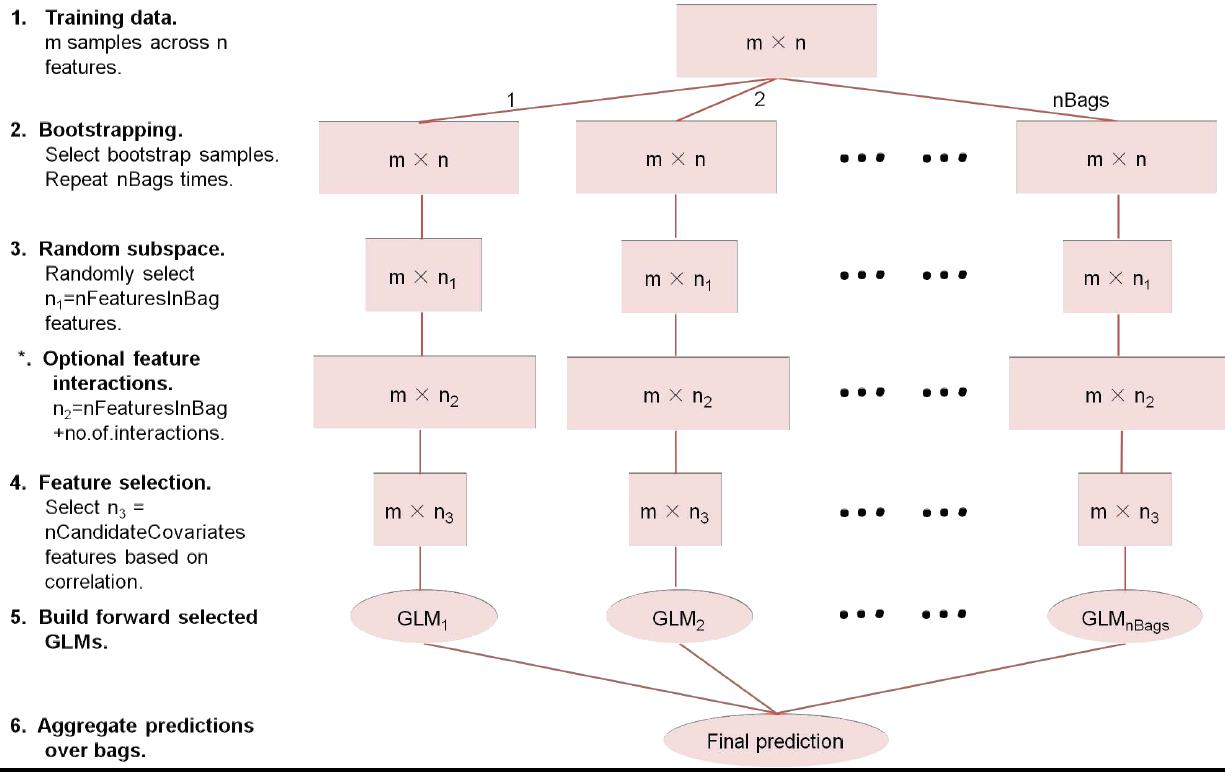
\includegraphics[width=0.9\textwidth]{images/RGLM.jpg}
	\caption{An overview of how RGLM works \cite{RGLM}}
	\label{fig:RGLM}
\end{figure}
Another technique we thought would be useful was using Random Generalized Linear Models. The way RGLM works is very similar to RF, however instead of training decision trees, RGLM trains generalized linear models. This is very nice because it takes the ensembling aspect of RF and combines it with a model that is more easily interpreted.
\subsection{Regression}
One issue we encountered with RGLM is that our code could not use factor variables for regression prediction. As such, the \(R_a^2\) value for our RGLM regression suffered. After running our analysis our five values ranged from .0174 to .0194 with an average of .0187. This is around the same as our initial linear regressions, and does not have strong predictive power.
\subsection{Classification}
Due to the binary nature of GLM classification, to classify NPV with RGLM, we decided to opt for classification into NPVs above and below the median. After running our analysis in a similar way to RF, our cross validated results had a minimum accuracy of .543, maximum accuracy of.560, and average of .557. This is not very much better than random guessing, which we would assume to be around .500. 
\section{Conclusion}
While the ability to predict mortgage loan NPV with the origination data was not as strong as we had initially assumed, we still proved that methods such as RF and RGLM outperform simple linear models. In the future, collating other quarters of data into the models as well as microeconomic and macroeconomic indicators may also help boost predictive power. 
\input biblio
\newpage
\section*{ACKNOWLEDGMENTS}
\addcontentsline{toc}{section}{Acknowledgments}
I would like to thank Dr. Yishi Wang for advising me throughout this project. Whether it was our weekly meetings, emails, or online meetings at either 8:30 PM or 9:00 AM, Dr. Wang has been unbelievably helpful this whole process. \\
\linebreak
I'd like to thank Dr. Ann  Stapleton for facilitating my learning of R,  Github, UNIX, among so many other technical skills. Dr. Stapleton also helped me learn other best practices for large software based projects. Without already having learned these skills working for Dr. Stapleton I would not have been able to widen the scope of this project to what it became.\\
\linebreak 
I'd like to thank my family and friends for supporting me through this project. Without you guys, I don't know if I could have done it.\\
\linebreak
I'd like to thank the Texas Advanced Computing Center (TACC) at The University of Texas at Austin for providing HPC resources that have contributed to the research results reported within this paper. URL: http://www.tacc.utexas.edu
%
% Biographical Sketch (Optional)

\end{document}
